\documentclass{fithesis}

\usepackage{lmodern}
\usepackage[czech]{babel}
\usepackage[utf8]{inputenc}
\usepackage{cmap}
\usepackage{graphicx}
\usepackage[T1]{fontenc} %formátuje české znaky - důležité
\usepackage[plainpages=false, pdfpagelabels]{hyperref}
\usepackage{hyperref}
%\usepackage{makeidx}
%\makeindex

%\bibliographystyle{unsrt}


%\makeindex
\thesistitle{Název}
\thesissubtitle{Diplomová práce}
\thesisstudent{Marek Tlačbaba}
\thesiswoman{false}
\thesisfaculty{fi}
\thesisyear{rok}
\thesisadvisor{vedoucí}


\begin{document}

\FrontMatter
\ThesisTitlePage

\begin{ThesisDeclaration}
Prohlášení\AdvisorName
\end{ThesisDeclaration}

\begin{ThesisThanks}
Poděkování
\end{ThesisThanks}

\begin{ThesisAbstract}
Abstrak
\end{ThesisAbstract}

\begin{ThesisKeyWords}
Klíčová slova
\end{ThesisKeyWords}


\MainMatter
\setcounter{secnumdepth}{4}
\tableofcontents

\chapter{Úvod}



\section{Vzorová kapitola}
\subsection{Vzorová podkapitola}

\begin{figure}[htp]
\centering
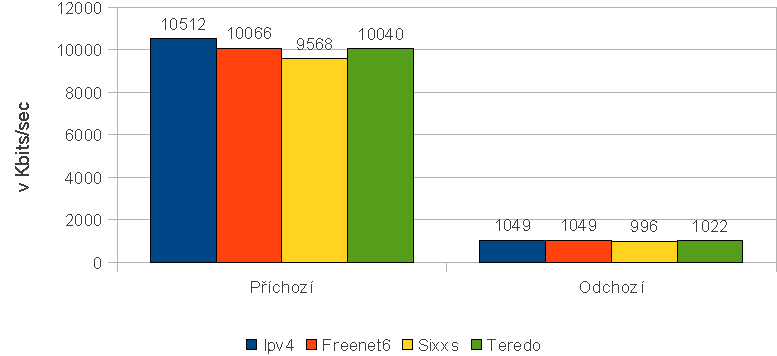
\includegraphics[width=340px]{images/bandwith.pdf}
\caption{Vzorový obrázek}
\end{figure}

\begin{itemize}
\item vzorový seznam
\end{itemize}


\begin{table}
\centering
\begin{tabular}{|p{3cm}|p{8cm}|}
\hline Sloupec 1 & Sloupec 2 \\
\hline Položka 2 & položka 2 \\
\hline
\end{tabular}
\caption{Vybrané skupinové adresy (převzato z \cite{satrapa-ipv6})}
\end{table}



%\printindex

\begin{thebibliography}{0}

\bibitem{satrapa-ipv6}
SATRAPA, P. \textit{IPv6 - Internetový protokol verze 6}. Praha : CZ.NIC, 2008.







\end{thebibliography}


\newpage
\appendix
\chapter{Položky seznamu}
asdfsadf

\chapter{Položky seznamu}
asdfsadf


\end{document}